%!TEX program = xelatex
% 完整编译: xelatex -> biber/bibtex -> xelatex -> xelatex
\documentclass[lang=cn,11pt,a4paper]{elegantpaper}

\title{LR语法分析程序的设计与实现}
\author{杨晨 \\学号2021212171}
\institute{北京邮电大学 计算机学院}

% \version{0.10}
\date{\zhtoday}

% 本文档命令
\usepackage{array}
\usepackage{xcolor}
\newcommand{\ccr}[1]{\makecell{{\color{#1}\rule{1cm}{1cm}}}}

\usepackage{fontspec}

% 设置代码样式
% 定义 Python 代码样式
\lstdefinestyle{pythonstyle}{
    language=Python,
    basicstyle=\ttfamily\small,
    backgroundcolor=\color{gray!10},
    commentstyle=\color{gray},
    keywordstyle=\color{blue},
    stringstyle=\color{green!60!black},
    showstringspaces=false,
    breaklines=true,
    numberstyle=\tiny\color{gray},
    frame=single,
    rulecolor=\color{black},
    captionpos=b,
    tabsize=4,
    morekeywords={as, with},
    keywordstyle=[2]\color{orange},
    keywordstyle=[3]\color{violet},
    keywordstyle=[4]\color{teal},
    keywordstyle=[5]\color{purple},
    keywordstyle=[6]\color{cyan!60!black}
}

\setmonofont{Courier New}  % 设置代码块中的字体

% 设置 Python 代码样式
\lstset{
    style=pythonstyle,
}

% 纯文本样式
\lstdefinelanguage{text}{
    basicstyle=\fontsize{7pt}{9pt}\ttfamily,
    keywordstyle=\fontsize{7pt}{9pt}\ttfamily,
    commentstyle=\fontsize{7pt}{9pt}\ttfamily,
    stringstyle=\fontsize{7pt}{9pt}\ttfamily,
    escapeinside={(*@}{@*)},
    showstringspaces=false,
    breaklines=true,
    breakatwhitespace=true,
    tabsize=4
}
\begin{document}



\maketitle
% \tableofcontents

\section{概述}

\subsection{实验内容}

编写语法分析程序,实现对算术表达式的语法分析。要求所分析算术表达式由如下的文法产生。

\label{grammar}
$$
\begin{aligned}
& E\rightarrow E+T | E-T | T \\
& T\rightarrow T*F | T/F | F \\
& F\rightarrow (E) | num
\end{aligned}
$$

要求在对输入的算术表达式进行分析的过程中,依次输出所采用的产生式。

编写LR语法分析程序,实验要求和实现方法要求如下:

\begin{enumerate}
    \item 构造识别该文法所有活前缀的DFA。
    \item 构造该文法的LR分析表。
    \item 编程实现算法4.3,构造LR分析程序。
\end{enumerate}

    
\subsection{开发环境}

\begin{itemize}
    \item Windows10
    \item PyCharm 2023.2.4 (Professional Edition)
\end{itemize}

\section{程序的功能模块划分}

\subsection{文法Grammar类}

\subsubsection{定义}

首先,考虑文法的特点,它的终结符和非终结符号,字母符号之间都具有互异、唯一的特点,所以可以用集合来存储,在后续遍历中,需要维护集合中元素的顺序,所以采用有序集合来存储。

其次,考虑产生式,一个非终结符号,可能会有多个右部产生式,同时,为了方便查找产生式,可以用字典来存储产生式,字典的键值是左部符号,对应的值是一个列表,包含这个符号的所有产生式,而LR分析中涉及到拓广文法,需要为产生式编号,维护产生式的顺序,所以采用有序字典来储存。

此外,还将使用一个有序字典,将编号和产生式对应起来,便于后续查询;用一个整数变量来记录文法中产生式的总个数

\begin{lstlisting}[language=Python]
from collections import OrderedDict
from ordered_set import OrderedSet
class Grammar:
    def __init__(self):
        self.non_terminals = OrderedSet()  # 非终结符
        self.terminals = OrderedSet()  # 终结符
        self.productions = OrderedDict()  # 产生式
        self.start_symbol = None  # 开始符号
        self.production_count = OrderedDict()  # 产生式编号
        self.count = 0  # 产生式个数
\end{lstlisting}

\lstinline{Grammar} 类的构造函数 \lstinline{__init__}初始化了文法对象的各个属性:
\begin{itemize}
    \item \lstinline{non_terminals} 是一个有序集合,用于存储非终结符(\lstinline{non-terminal})。
    \item \lstinline{terminals} 是一个有序集合,用于存储终结符(\lstinline{terminal})。
    \item \lstinline{productions} 是一个有序字典,用于存储产生式(\lstinline{production})。字典的键是非终结符,值是该非终结符对应的产生式列表,其中列表中每个元素是一个字符串,对应一个产生式。
    \item \lstinline{start_symbol} 是一个变量,用于文法存储起始符号。
    \item \lstinline{production_count}是一个有序字典,用于将产生式编号和产生式对应起来,其中字典的键是编号,值是一个字典(产生式左部:产生式右部)
    \item \lstinline{count}是一个整数,代表当前文法里,产生式的个数
\end{itemize}

\subsubsection{添加产生式}

由于我们通常约定,终结符号是大写字母,而非终结符合是小写字母,所以可以利用这个特点来填充终结符号集合和非终结符号集合

而产生式的右部长度不能确定,为了简单起见,采用一次插入一个产生式的方法,即如果产生式是形如
$$
\begin{aligned}
& E\rightarrow E+T | E-T | T \\
\end{aligned}
$$
这样的形式,那么则需要调用3次添加函数
$$
\begin{aligned}
& add\_production('E', 'E+T') \\
& add\_production('E', 'E-T') \\
& add\_production('E', 'T')
\end{aligned}
$$

\begin{lstlisting}[language=Python]
# 添加产生式,参数为左部和右部
def add_production(self, non_terminal, production):
    if non_terminal not in self.productions:
        self.productions[non_terminal] = []

    self.productions[non_terminal].append(production)
    self.non_terminals.add(non_terminal)

    if production == "num":
        self.terminals.add("num")
    else:
        for symbol in production:
            if symbol.isalpha() and not symbol.islower():  # 是大写字母
                self.non_terminals.add(symbol)
            else:
                self.terminals.add(symbol)
\end{lstlisting}

\lstinline{add_production}方法用于向文法中添加产生式。它接受两个参数:\lstinline{non_terminal}(非终结符)和 \lstinline{production}(产生式)。该方法将产生式添加到相应的非终结符的产生式列表中,并更新 \lstinline{non_terminals} 和 \lstinline{terminals} 集合。

\subsubsection{拓广文法}

下面的方法实现了拓广文法,即对于文法$G=(N,T,P,S)$,生成与其等价的文法$G'=(N\cup \{S'\},T,P\cup\{S'\rightarrow S\},S')$。并打印拓广文法

\begin{lstlisting}[language=Python]
# 拓广文法并打印
def expand_grammar(self):
    new_non_terminals = OrderedSet()
    new_productions = OrderedDict()
    new_start_symbol = self.start_symbol + "'"
    new_non_terminals.add(new_start_symbol)
    new_productions[new_start_symbol] = [self.start_symbol]
    for non_terminal in self.non_terminals:
        new_non_terminals.add(non_terminal)
        new_productions[non_terminal] = self.productions[non_terminal]
    self.non_terminals = new_non_terminals
    self.productions = new_productions
    self.start_symbol = new_start_symbol
    for non_terminal in self.non_terminals:
        right_list = self.productions[non_terminal]
        for right_str in right_list:
            key = {non_terminal: right_str}
            self.production_count[self.count] = key
            self.count += 1
    for i in range(self.count):
        for key in self.production_count[i]:
            print("{:2} -> ".format(key), end="")
            print("{:5}".format(self.production_count[i][key]), end="")
        print("{:10}".format(i))
    print()
\end{lstlisting}


\lstinline{eliminate_left_recursion}方法用于消除文法中的左递归。


这段代码实现了一个拓广文法的函数。它通过在原始文法的基础上添加额外的产生式和非终结符来拓广文法。具体步骤如下:
\begin{enumerate}
    \item 创建新的非终结符集合和产生式字典,用于存储拓广后的文法。
    \item 将原始文法的起始符号加上撇号,作为新的起始符号。
    \item 将原始文法的起始符号对应的产生式设置为新的起始符号。
    \item 将原始文法中的非终结符号和对应的产生式添加到拓广后的文法中。
    \item 更新原始文法的非终结符集合和产生式字典为拓广后的集合。
    \item 遍历拓广后的非终结符集合中的每个非终结符,获取对应的产生式列表。
    \item 为每个产生式创建一个新的键值对,将其添加到产生式计数器中。
    \item 打印拓广后的产生式,包括非终结符和对应的产生式字符串。
\end{enumerate}

通过这些步骤,该函数能够将原始文法拓广为一个包含额外产生式的新文法,并将拓广后的产生式打印出来。

\subsubsection{根据产生式查找编号}

在设计拓广文法的产生式时,字典的键是编号,值是产生式,但是在LR(1)的规约动作时,我们需要输出选择的是哪个编号的产生式进行规约,因此,需要一个能通过产生式查找到对应编号的方法

\begin{lstlisting}
 # 根据产生式左部和右部查找产生式编号
def find_production(self, left, right):
    for i in range(self.count):
        if (
            left in self.production_count[i]
            and right in self.production_count[i].values()
        ):
            return str(i)
    return None
\end{lstlisting}

这段代码实现了一个函数,用于根据给定的产生式左部和右部,在产生式字典中查找对应的产生式编号。

函数名为 \lstinline{find_production},接受两个参数 \lstinline{left} 和 \lstinline{right},分别表示产生式的左部和右部。

使用 \lstinline{for} 循环遍历产生式计数器中的每个产生式编号 \lstinline{i}。
在循环内部,使用条件判断语句检查以下两个条件:
\begin{itemize}
    \item \lstinline{left} 是否存在于第 \lstinline{i} 个产生式的键中。
    \item \lstinline{right} 是否存在于第 \lstinline{i} 个产生式的值中(即右部)。
\end{itemize}

如果上述两个条件都满足,则表示找到了对应的产生式,返回该产生式的编号,使用 \lstinline{str(i)} 将其转换为字符串形式。

如果循环结束后仍然没有找到匹配的产生式,即没有满足条件的产生式,返回 \lstinline{None} 表示未找到。

这个函数的作用是根据给定的产生式左部和右部,查找对应的产生式编号。它通过遍历产生式计数器中的每个产生式进行查找,当找到匹配的产生式时,返回该产生式的编号。如果没有找到匹配的产生式,则返回 \lstinline{None} 表示未找到。

\subsubsection{文法格式化输出}

为了便于观察和调试,我还设计了将文法按照标准格式进行输出的方法

\begin{lstlisting}
# 输出文法
def print_grammar(self):
    for non_terminal in self.productions:
        print(non_terminal + " -> " + " | ".join(self.productions[non_terminal]))
    print()
\end{lstlisting}

可以在需要进行验证,或者调试的地方调用该方法,查看当前的文法

\subsection{识别项目集规范族的DFA}

\subsubsection{定义}

考虑到状态集合中,每个状态都是互不相同的,且我们需要通过状态编号来获取该状态的内容,所以用字典来存储。而对于每个状态,我们希望它是有序的,这样便于在后续的DFA中进行广度优先遍历

状态和状态之间,是通过符号来转移的,所以转移边集一定是一个二维的数据结构,考虑到在最终的LR分析时,我们有查询转移边的需要,所以用二维字典来存储

此外,还需要一个整数变量来记录当前状态集中状态的个数

\begin{lstlisting}
class DFA:
    def __init__(self):
        self.states = {0: OrderedSet()}  # 所有状态的集合,key为状态编号,value为状态
        self.transitions = {}  # 转移边集,二维字典,key为状态编号,value为字典,字典的key为下一个状态编号,value为转移符号
        self.count_state = 0  # 状态个数
\end{lstlisting}

这段代码定义了一个DFA(Deterministic Finite Automaton,确定有限状态自动机)类。下面是对代码的详细分析:
\begin{enumerate}
    \item \lstinline{class DFA} 定义了一个名为DFA的类。
    \item \lstinline{def __init__(self)} 定义了类的构造函数,用于初始化DFA的属性。
    \item \lstinline{states}是一个字典,用于存储DFA的状态集合。初始时,只有一个状态0,并且对应的值是一个空的有序集合(OrderedSet)。状态编号用作字典的键,状态本身存储在对应键的值中。
    \item \lstinline{transitions}是一个二维字典,用于存储DFA的转移边集。外层字典的键是状态编号,对应的值是一个字典。内层字典的键是下一个状态的编号,对应的值是转移符号。
    \item \lstinline{count_state}是一个整数,用于记录状态的个数。初始时,状态个数为0。
\end{enumerate}

通过这些属性,DFA类可以表示和存储有限状态自动机的状态集合、转移边集和状态个数。

\subsubsection{计算First集}

构建某个子串的FIRST集,方法如下

首先获取子串的首字符$s[0]$,如果$s[0]$是终结符或$\$$符,则直接返回$s[0]$

否则,令$s[0] = A$,对于任意产生式$A\rightarrow\alpha$,若$\alpha\not=\varepsilon$,设该产生式为:

$$
    A\rightarrow Y_1 | Y_2\ldots Y_k
$$

遍历产生式右部的每一个$Y_i$,如果:

\begin{itemize}
    \item $Y_i$是终结符,则$\alpha$的FIRST集中增加$Y_i$
    \item $Y_i$是非终结符,且不同于左部符号(防止无限递归),如果没有求出它的FIRST集,则递归求解。之后,$\alpha$的FIRST集并上$Y_i$的FIRST集。
\end{itemize}

最后,$A$的FIRST集为各个候选式的FIRST集的并,也就是待求子串的FIRST集。

\begin{lstlisting}
# 计算first集,是计算LR1自动机闭包的一部分
def get_first(self, grammar, s):
    if s[0] in grammar.terminals or s == "$":
        return s[0]
    right_list = grammar.productions[s[0]]
    first_str = None
    for right_str in right_list:
        if right_str[0] in grammar.terminals:
            first_str = right_str[0]
        elif right_str == "num":
            first_str = "num"
        elif right_str[0] == s[0]:
            continue
        else:
            first_str = self.get_first(grammar, right_str[0])
    return first_str
\end{lstlisting}

这段代码,用于计算LR1自动机闭包中的符号串的first集合。
\begin{enumerate}
    \item \lstinline{get_first}方法接受两个参数:\lstinline{grammar}表示文法规则,\lstinline{s}表示一个符号串。
    \item 如果符号串\lstinline{s}的第一个字符是终结符或者\lstinline{s}本身是终结符\lstinline{"$"},直接返回该字符。
    \item 从文法规则的产生式中获取以\lstinline{s[0]}为产生式左侧的所有产生式的右侧部分的列表。
    \item 初始化一个变量\lstinline{first_str}为\lstinline{None},用于存储计算得到的\lstinline{first}集合。
    \item 遍历产生式右侧部分的列表:
    \begin{itemize}
        \item 如果产生式右侧部分的首字符是终结符,则将该字符赋值给\lstinline{first_str}。
        \item 如果产生式右侧部分为字符串\lstinline{"num"},则将\lstinline{"num"}赋值给\lstinline{first_str}。
        \item 如果产生式右侧部分的首字符与\lstinline{s}的首字符相同,跳过当前循环,继续下一个产生式。
        \item 如果以上条件都不满足,则递归调用\lstinline{get_first}方法,传入产生式右侧部分的首字符,计算其\lstinline{first}集合,并将结果赋值给\lstinline{first_str}。
    \end{itemize}
    \item 返回计算得到的\lstinline{first}集合。
\end{enumerate}


总体来说,该方法根据给定的文法规则和符号串,计算了符号串的\lstinline{first}集合,用于LR1自动机中闭包的计算。

\subsubsection{计算闭包}

构造LR(1)项目集的闭包,方法如下

\begin{enumerate}
    \item 初始化$closure(I)\leftarrow I$;
    \item 对于$[A\rightarrow \alpha\cdot B\beta, a]\in closure(I)$,若$B\rightarrow\eta\in \mathrm P$,则$\forall b\in FIRST(\beta a)$,使$closure(I)\leftarrow closure(I)\cup [B\rightarrow \cdot \eta,b]$;
    \item 重复2直至$closure(I)$不再增大为止。
\end{enumerate}


\begin{lstlisting}
# 计算LR1自动机的闭包
def get_closure(self, grammar, state):
    closure = state
    for item in state:
        left = item[0][0]
        right_str = item[0][1]
        for ii in range(len(item[1])):
            look_ahead = str(item[1][ii])
            for i in range(len(right_str)):
                if right_str[i] == "·" and i + 1 < len(right_str):
                    if right_str[i + 1] in grammar.non_terminals:  # ·后面是非终结符
                        for production in grammar.productions[right_str[i + 1]]:
                            if i + 1 == len(right_str) - 1:  # ·在倒数第二个位置
                                str_ahead = look_ahead
                            else:
                                str_ahead = right_str[i + 2 :] + look_ahead
                            tmp = (
                                (right_str[i + 1], "·" + production),
                                tuple(self.get_first(grammar, str_ahead)),
                            )
                            if tmp not in closure:
                                closure.add(tmp)
    return closure
\end{lstlisting}

这段代码是DFA类中的一个方法\lstinline{get_closure},用于计算LR1自动机中给定状态的闭包。

\begin{enumerate}
    \item \lstinline{get_closure}方法接受两个参数:\lstinline{grammar}表示文法规则,\lstinline{state}表示一个状态。
    \item 初始化闭包为给定状态。
    \item 遍历状态中的每个项目:
    \begin{itemize}
        \item 获取产生式左侧的符号和右侧的符号串。
        \item 遍历项目的每个向前看符号。
        \item 如果当前字符是"·"且不是最后一个字符,并且"·"后面的字符是非终结符:
        \begin{itemize}
            \item 遍历非终结符的产生式。
            \item 根据向前看符号和"·"后面的字符之后的符号串和向前看符号计算得到新的向前看符号集合。
            \item 创建一个新的项目,其中产生式左侧为非终结符后跟"·"和产生式右侧,新的向前看符号集合为上面计算得到的first集合。
            \item 如果新的项目不在闭包中,将其添加到闭包。
        \end{itemize}
    \end{itemize}
    \item 返回闭包。
\end{enumerate}

该方法通过扩展状态中的项目,并根据后继非终结符的产生式生成新的项目,直到闭包不再增大为止。在计算闭包的过程中,会根据新的向前看符号和后继符号串计算得到新的向前看符号集合,并将新的项目添加到闭包中。这是构建LR1自动机中的闭包集合的重要步骤。

\subsubsection{合并状态中的产生式}

在刚刚的计算闭包方法中,会产生许多产生式相同,但是向前看符号不同的元组,为了便于后面的分析,可以将状态进行化简

\begin{lstlisting}
# 对于相同的左部产生式,合并look_ahead
def merge(self, state):
    lst = state
    merged_dict = {}

    for item in lst:
        key = item[0]
        value = list(item[1])

        if key in merged_dict:
            for i in range(len(value)):
                if value[i] not in merged_dict[key]:
                    merged_dict[key].append(value[i])
        else:
            merged_dict[key] = value

    merged_list = [(key, value) for key, value in merged_dict.items()]
    new_states = OrderedSet()
    for i in range(len(merged_list)):
        tmp = (
            (merged_list[i][0][0], merged_list[i][0][1]),
            tuple(merged_list[i][1]),
        )
        new_states.add(tmp)
    return new_states
\end{lstlisting}

这段代码是DFA类中的一个方法\lstinline{merge},用于合并具有相同左部产生式的状态的展望符(\lstinline{look_ahead})。以下是对代码的简要概括:
\begin{enumerate}
    \item \lstinline{merge}方法接受一个参数\lstinline{state},表示一个状态。
    \item 初始化一个空字典\lstinline{merged_dict},用于存储合并后的向前看符号。
    \item 遍历状态中的每个项目:
    \begin{itemize}
        \item 将项目的左部产生式作为字典的键,展望符作为字典的值。
        \item 如果字典中已存在相同的左部产生式键,将当前向前看符列表中不在字典值中的展望符添加到字典值中。
        \item 如果字典中不存在相同的左部产生式键,将当前向前看符列表作为字典值。
    \end{itemize}
    \item 将字典转换为包含键值对的元组列表\lstinline{merged_list}。
    \item 初始化一个有序集合\lstinline{new_states},用于存储合并后的状态。
    \item 遍历合并后的列表\lstinline{merged_list}:
    \begin{itemize}
        \item 创建一个新的项目,其中左部产生式为元组的第一个元素,向前看符为元组的第二个元素。
        \item 将新的项目添加到\lstinline{new_states}中。
    \end{itemize}
    \item 返回合并后的状态\lstinline{new_states}。
\end{enumerate}

该方法用于合并具有相同左部产生式的状态中的向前看符,将向前看符列表合并为一个唯一的向前看符列表。这是在构建LR1自动机过程中对状态进行优化和合并的一步。

\subsubsection{状态之间建边}

在广度优先遍历的过程中,我们需要为状态和状态之间的转移建立边,边权为转移符号

\begin{lstlisting}
# 添加边,参数为状态编号,下一个状态编号,转移符号
def add_edge(self, start_vertex, end_vertex, weight):
    if start_vertex not in self.transitions:
        self.transitions[start_vertex] = {}
    self.transitions[start_vertex][end_vertex] = weight
\end{lstlisting}

这段代码是DFA类中的一个方法\lstinline{add_edge},用于向LR1自动机中添加转移边。以下是对代码的简要概括:

\begin{enumerate}
    \item \lstinline{add_edge}方法接受三个参数:\lstinline{start_vertex}表示起始状态的编号,\lstinline{end_vertex}表示下一个状态的编号,\lstinline{weight}表示转移符号。
    \item 首先检查起始状态是否已存在于转移字典\lstinline{transitions}中。
    \item 如果起始状态不存在于转移字典中,创建一个空字典作为起始状态的条目。
    \item 将下一个状态和转移符号添加到起始状态的条目中,以建立起始状态到下一个状态的转移边。
\end{enumerate}

该方法用于在LR1自动机中添加转移边,它将起始状态、下一个状态和转移符号作为参数,并将转移信息存储在转移字典\lstinline{transitions}中。这是构建LR1自动机中状态之间转移关系的重要步骤。

\subsubsection{状态格式化输出}

为了便于观察和调试,我还设计了将状态按照标准格式进行输出的方法

可以打印指定编号的状态,也可以将整个DFA打印出来

\begin{lstlisting}
# 打印状态number
def print_state(self, number):
    for item in self.states[number]:
        print(f"{item[0][0]} -> {item[0][1]} , {'|'.join(list(item[1]))}")

# 打印整个自动机
def show_dfa(self):
    for num in range(self.count_state):
        print("状态I{}:".format(num))
        self.print_state(num)
        if num in self.transitions:
            for neighbor in self.transitions[num]:
                print(
                    "--- {} ---> 状态I{}".format(
                        self.transitions[num][neighbor], neighbor
                    )
                )
        print()
\end{lstlisting}

可以在需要进行验证,或者调试的地方调用该方法,查看当前的状态和状态集

\subsection{LR1分析器}

\subsubsection{定义}

对于LR1语法分析,需要创建LR1的自动机

对于预测分析表,由于它是一个二维表格,我们仍然可以用字典来存储,其中键是一个二元元组,包括状态编号和符号,值是采取的动作(str类型)。

\begin{lstlisting}
class LR1Parser:
    def __init__(self):
        self.DFA = DFA()  # LR1自动机
        self.analysis_table = {}  # 分析表
\end{lstlisting}

\lstinline{LL1Parser} 类的构造函数 \lstinline{__init__}初始化了文法对象的各个属性:
\begin{itemize}
    \item \lstinline{DFA } 是DFA类,代表LR1的自动机
    \item \lstinline{analysis_table} 是一个字典,用于存储预测分析表
\end{itemize}

\subsubsection{初始化I0状态}

I0的初始化,就是将
$$
\begin{aligned}
& ((E', \cdot E), (\$))
\end{aligned}
$$

加入其中,然后,计算闭包,合并产生式

注意要将\lstinline{count_state}加1

\begin{lstlisting}
# 初始化I0状态
def compute_first(self, grammar):
    right_str = "·" + grammar.production_count[0][grammar.start_symbol]
    tmp = ((grammar.start_symbol, right_str), tuple("$"))
    self.DFA.states[0].add(tmp)
    self.DFA.count_state += 1
    self.DFA.states[0] = self.DFA.get_closure(grammar, self.DFA.states[0])
    self.DFA.states[0] = self.DFA.merge(self.DFA.states[0])
\end{lstlisting}

\subsubsection{计算LR(1)自动机}

下面是构造识别给定文法的所有活前缀的DFA

\begin{lstlisting}
# 计算LR1自动机
def compute_lr1_automaton(self, grammar, number=0):
    if number == 0:  # 初始化I0状态
        self.compute_first(grammar)
    if number == self.DFA.count_state:  # 计算完毕
        self.DFA.show_dfa()
        return
    state = self.DFA.states[number]
    classified_dict = OrderedDict()  # 按照·后面的字符分类
    for item in state:
        dot_index = item[0][1].find("·")
        if dot_index != -1 and dot_index + 1 < len(item[0][1]):
            key = item[0][1][dot_index + 1]
            if key == "n":
                key = "num"
            if key not in classified_dict:
                classified_dict[key] = OrderedSet()
            classified_dict[key].add(item)

    for k, v in classified_dict.items():
        tmp_state = OrderedSet()
        for tpl in v:
            left = tpl[0][0]
            right_str = tpl[0][1]
            dot_index = right_str.find("·")
            new_right_str = ""
            if right_str[dot_index + 1 :] == "num":
                new_right_str = "num·"
            elif dot_index != -1 and dot_index + 1 < len(right_str):
                new_right_str = (
                    right_str[:dot_index]
                    + right_str[dot_index + 1]
                    + "·"
                    + right_str[dot_index + 2 :]
                )
            tmp = ((left, new_right_str), tpl[1])
            tmp_state.add(tmp)
        tmp_state = self.DFA.get_closure(grammar, tmp_state)
        tmp_state = self.DFA.merge(tmp_state)
        if tmp_state not in self.DFA.states.values():
            self.DFA.states[self.DFA.count_state] = tmp_state
            self.DFA.add_edge(number, self.DFA.count_state, k)
            self.DFA.count_state += 1
        else:
            for key, value in self.DFA.states.items():
                if value == tmp_state:
                    self.DFA.add_edge(number, key, k)

    self.compute_lr1_automaton(grammar, number + 1)
\end{lstlisting}

这段代码实现了LR(1)自动机的构建过程。它接受一个文法作为输入,并根据该文法构建LR(1)自动机。以下是对代码的简要概括:
\begin{enumerate}
    \item \lstinline{compute_lr1_automaton} 是一个递归函数,它接受三个参数:\lstinline{self}(指向类自身的引用)、\lstinline{grammar}(文法)和可选的 \lstinline{number}(用于追踪自动机的状态编号)。
    \item 如果 \lstinline{number} 等于0,表示正在初始化I0状态,这时调用 \lstinline{compute_first} 函数初始化I0状态。
    \item 如果 \lstinline{number} 等于自动机的状态数(即已经计算完毕),则打印整个自动机并返回。
    \item 获取当前状态 \lstinline{number} 对应的项目集合,并按照 $\cdot$ 后面的字符进行分类。
    \item 创建一个临时状态集合 \lstinline{tmp_state}。对于分类中的每个项目,找到·的位置,并根据情况生成新的右部字符串。创建一个新的项目,更新右部字符串,并将其添加到临时状态集合 \lstinline{tmp_state} 中。
    \item 调用 \lstinline{get_closure} 函数计算 \lstinline{tmp_state} 的闭包,调用 \lstinline{merge} 函数合并 \lstinline{tmp_state} 中的项目。
    \item 如果合并后的状态集合不在自动机的已有状态集合中,则将其添加为一个新的状态,并建立从当前状态到新状态的边,边的标签为分类的字符。
    \item 如果合并后的状态集合已经存在于自动机的状态集合中,则建立从当前状态到已存在状态的边。
    \item 递归调用 \lstinline{compute_lr1_automaton},并将 \lstinline{number} 值加1。
    \item 最终完成自动机的构建过程。
\end{enumerate}


\subsubsection{算法4.9 构造分析预测表}

\lstinline{compute_analysis_table(self, grammar)}函数通过 LR(1)项目集规范族构造一个LR分析表

\begin{lstlisting}
# 计算分析表,教材算法4.9
def compute_analysis_table(self, grammar):
    # 初始化分析表
    for num in range(self.DFA.count_state):
        self.analysis_table[num] = {}
        for terminal in grammar.terminals:
            self.analysis_table[num][terminal] = None
        self.analysis_table[num]["$"] = None
        for non_terminal in grammar.non_terminals:
            self.analysis_table[num][non_terminal] = None

    for num in range(self.DFA.count_state):
        if num in self.DFA.transitions:  # 有出边
            for neighbor in self.DFA.transitions[num]:
                if (
                    self.DFA.transitions[num][neighbor] in grammar.non_terminals
                ):  # 边是非终结符,goto下一个状态
                    self.analysis_table[num][
                        self.DFA.transitions[num][neighbor]
                    ] = str(neighbor)
                else:  # 边是终结符,action为Shift,并转移到下一个状态
                    self.analysis_table[num][
                        self.DFA.transitions[num][neighbor]
                    ] = "S" + str(neighbor)
        for item in self.DFA.states[num]:
            if item[0][1][-1] == "·":  # 产生式是规约项
                if item[0][0] == grammar.start_symbol:  # 产生式是开始符号
                    self.analysis_table[num]["$"] = "ACC"
                else:  # 产生式不是开始符号
                    for look_ahead in item[1]:
                        self.analysis_table[num][
                            look_ahead
                        ] = "R" + grammar.find_production(
                            item[0][0], item[0][1][0:-1]
                        )
    print("分析表:")
    print(
        "状态\t{}{}{}{}".format(
            "\t" * (int)(len(grammar.terminals) + 1),
            "action",
            "\t" * (int)(len(grammar.terminals) + 1),
            "GOTO",
        )
    )
    print("\t", end="")
    for terminal in grammar.terminals:
        print(terminal + "\t\t", end="")
    print("$\t\t", end="")
    for non_terminal in grammar.non_terminals:
        if non_terminal != grammar.start_symbol:
            print(non_terminal + "\t\t", end="")
    print()
    for num in range(self.DFA.count_state):
        print("{}\t".format(num), end="")
        for terminal in grammar.terminals:
            if self.analysis_table[num][terminal] is None:
                print("\t\t", end="")
            else:
                print(self.analysis_table[num][terminal] + "\t\t", end="")
        if self.analysis_table[num]["$"] is None:
            print("\t\t", end="")
        else:
            print(self.analysis_table[num]["$"] + "\t\t", end="")
        for non_terminal in grammar.non_terminals:
            if non_terminal != grammar.start_symbol:
                if self.analysis_table[num][non_terminal] is None:
                    print("\t\t", end="")
                else:
                    print(self.analysis_table[num][non_terminal] + "\t\t", end="")
        print()
    print()

\end{lstlisting}

这段代码是一个计算分析表的方法。它基于教材算法4.9实现。分析表用于LR分析器,在语法分析过程中帮助确定下一步的操作。代码首先初始化分析表,然后根据DFA的状态和转移关系填充表格。

对于有出边的状态,如果边是非终结符,则在分析表的对应位置记录下一个状态(goto表);如果边是终结符,则记录为"Shift"并转移到下一个状态(action表)。

对于规约项,即产生式的右部已经完全规约到左部的项,如果产生式是开始符号,则在分析表的"\$"位置记录为"ACC"(接受状态);如果产生式不是开始符号,则根据向前看符(lookahead)在分析表中记录规约动作(action表)。

最后,代码输出打印了计算得到的分析表。

\subsubsection{算法4.2 LR(1)预测分析}

\lstinline{parse(self, grammar, input_string)}函数实现对一个字符串进行LR(1)分析,并给出分析的结果

\begin{lstlisting}
# 分析输入串,教材算法4.3
def parse(self, grammar, input_string):
    print("{:50}".format("Stack"), "\t{:40}".format("Input"), "\tAction")
    stack = [[0, "~"]]
    ptr = 0
    while True:
        # print("{:30}".format("Stack"), "\t{:30}".format("Input") + "$")
        pit_state = " ".join(str(stack[i][0]) for i in range(len(stack)))
        pit_symbol = " ".join(
            "{:>2}".format(str(stack[i][1]))
            if stack[i][0] > 9
            else "{:>1}".format(str(stack[i][1]))
            for i in range(len(stack))
        )
        print("State:  {:42}".format(pit_state))
        print(
            "Symbol: {:42}".format(pit_symbol),
            "\t{:40}".format(input_string[ptr:]),
            end="",
        )
        now_string = ""
        if ptr == len(input_string):  # 输入串已经读完
            now_string = "$"
        elif input_string[ptr].isdigit():  # 输入串中的符号是数字
            now_string = "num"
        else:
            now_string = input_string[ptr]
        if self.analysis_table[stack[-1][0]][now_string] is None:
            print("\t\033[91m error(s) \033[0m")
            break
        elif self.analysis_table[stack[-1][0]][now_string] == "ACC":
            print("\t\033[92mAcc!\033[0m", end="")
            break
        elif self.analysis_table[stack[-1][0]][now_string][0] == "S":  # 移进Shift
            next_num = int(self.analysis_table[stack[-1][0]][now_string][1:])
            print("\tShift {}".format(next_num))
            stack.append([next_num, input_string[ptr]])
            ptr += 1
        elif self.analysis_table[stack[-1][0]][now_string][0] == "R":  # 规约Reduce
            production_num = int(
                self.analysis_table[stack[-1][0]][now_string][1:]
            )  # 记录产生式编号,将产生式右部弹出,左部压入
            left = list(grammar.production_count[production_num].keys())[0]
            right = list(grammar.production_count[production_num].values())[0]
            if right == "num":
                pop_num = 1
            else:
                pop_num = len(right)
            print("\treduce by {} -> {}".format(left, right))
            for i in range(pop_num):
                stack.pop()
            stack.append([int(self.analysis_table[stack[-1][0]][left]), left])
        print()
\end{lstlisting}

这段代码是用于分析输入串的方法,基于教材算法4.3实现。它使用LR分析表对输入串进行逐步分析。算法通过一个栈和一个指针来模拟分析的过程。代码首先初始化栈,将初始状态0和符号"~"压入栈中。然后,通过循环进行分析,每次迭代输出当前的栈状态、输入串和执行的动作。

在每次迭代中,代码首先检查输入串是否已经读取完毕,如果是,则将当前符号设置为"\$";如果当前符号是数字,则将其设置为"num"。然后,根据栈顶状态和当前符号,在分析表中查找相应的动作。
\begin{itemize}
    \item 如果在分析表中找不到对应的动作,则输出错误信息并终止分析。
    \item 如果分析表中的动作是"ACC"(接受状态),则输出"Acc!"表示成功完成分析。
    \item 如果分析表中的动作是以"S"开头的字符串(移进动作),则将该状态压入栈中,并将指针向前移动一位。
    \item 如果分析表中的动作是以"R"开头的字符串(规约动作),则根据产生式的编号进行规约操作,将产生式右部弹出栈,将产生式左部和相应状态压入栈中。
\end{itemize}

在每次迭代结束后,打印当前的栈状态、符号、输入串和执行的动作。如果成功接受输入串,则输出"Acc!"表示成功完成分析。如果发生错误,输出错误信息并终止分析。

这段代码实现了LR分析器的核心逻辑,通过栈和分析表的操作,可以对输入串进行逐步的推导和分析,判断其是否符合给定的文法规则。

\section{使用说明}

\textbf{直接运行\lstinline{Gramma_LR.py}即可}

下面是\lstinline{main}函数中,每条语句的逐行分析


\subsection{输入给定文法}
在\lstinline{Gramma_LR.py}中,首先将给定文法添加到文法类中,便于后续分析
\begin{lstlisting}
grammar = Grammar()
grammar.add_production("E", "E+T")
grammar.add_production("E", "E-T")
grammar.add_production("E", "T")
grammar.add_production("T", "T*F")
grammar.add_production("T", "T/F")
grammar.add_production("T", "F")
grammar.add_production("F", "(E)")
grammar.add_production("F", "num")
grammar.start_symbol = "E"
print("原文法")
grammar.print_grammar()

print("Non-terminals:", grammar.non_terminals)
print("Terminals:", grammar.terminals)
print("Start symbol:", grammar.start_symbol)
print("Productions:", grammar.productions, "\n")
\end{lstlisting}

打印出的文法类Grammar的情况如下
\begin{lstlisting}[language=text]
原文法
E -> E+T | E-T | T
T -> T*F | T/F | F
F -> (E) | num

Non-terminals: OrderedSet(['E', 'T', 'F'])
Terminals: OrderedSet(['+', '-', '*', '/', '(', ')', 'num'])
Start symbol: E
Productions: OrderedDict([('E', ['E+T', 'E-T', 'T']), ('T', ['T*F', 'T/F', 'F']), ('F', ['(E)', 'num'])]) 
\end{lstlisting}

\subsection{拓广文法}

之后,需要将文法改写为拓广文法
\begin{lstlisting}
print("拓广文法后")
grammar.expand_grammar()

print("Non-terminals:", grammar.non_terminals)
print("Terminals:", grammar.terminals)
print("Start symbol:", grammar.start_symbol)
print("Productions:", grammar.productions, "\n")
\end{lstlisting}

输出新的拓广文法

\begin{lstlisting}[language=text]
拓广文法后
E' -> E             0
E  -> E+T           1
E  -> E-T           2
E  -> T             3
T  -> T*F           4
T  -> T/F           5
T  -> F             6
F  -> (E)           7
F  -> num           8

Non-terminals: OrderedSet(["E'", 'E', 'T', 'F'])
Terminals: OrderedSet(['+', '-', '*', '/', '(', ')', 'num'])
Start symbol: E'
Productions: OrderedDict([("E'", ['E']), ('E', ['E+T', 'E-T', 'T']), ('T', ['T*F', 'T/F', 'F']), ('F', ['(E)', 'num'])])  
\end{lstlisting}

\subsection{计算DFA}

准备工作完毕后,开始进行LR(1)分析。首先需要构造LR(1)项目集规范族及识别其所有活前缀的DFA

\begin{lstlisting}
lr1_parser = LR1Parser()
print("计算LR1自动机:")
lr1_parser.compute_lr1_automaton(grammar)
\end{lstlisting}

整个DFA结果如下

\begin{lstlisting}[language = text]
计算LR1自动机:
状态I0:
E' -> ·E , $
E -> ·E+T , $|+|-
E -> ·E-T , $|+|-
E -> ·T , $|+|-
T -> ·T*F , $|+|-|*|/
T -> ·T/F , $|+|-|*|/
T -> ·F , $|+|-|*|/
F -> ·(E) , $|+|-|*|/
F -> ·num , $|+|-|*|/
--- E ---> 状态I1
--- T ---> 状态I2
--- F ---> 状态I3
--- ( ---> 状态I4
--- num ---> 状态I5

状态I1:
E' -> E· , $
E -> E·+T , $|+|-
E -> E·-T , $|+|-
--- + ---> 状态I6
--- - ---> 状态I7

状态I2:
E -> T· , $|+|-
T -> T·*F , $|+|-|*|/
T -> T·/F , $|+|-|*|/
--- * ---> 状态I8
--- / ---> 状态I9

状态I3:
T -> F· , $|+|-|*|/

状态I4:
F -> (·E) , $|+|-|*|/
E -> ·E+T , )|+|-
E -> ·E-T , )|+|-
E -> ·T , )|+|-
T -> ·T*F , )|+|-|*|/
T -> ·T/F , )|+|-|*|/
T -> ·F , )|+|-|*|/
F -> ·(E) , )|+|-|*|/
F -> ·num , )|+|-|*|/
--- E ---> 状态I10
--- T ---> 状态I11
--- F ---> 状态I12
--- ( ---> 状态I13
--- num ---> 状态I14

状态I5:
F -> num· , $|+|-|*|/

状态I6:
E -> E+·T , $|+|-
T -> ·T*F , $|+|-|*|/
T -> ·T/F , $|+|-|*|/
T -> ·F , $|+|-|*|/
F -> ·(E) , $|+|-|*|/
F -> ·num , $|+|-|*|/
--- T ---> 状态I15
--- F ---> 状态I3
--- ( ---> 状态I4
--- num ---> 状态I5

状态I7:
E -> E-·T , $|+|-
T -> ·T*F , $|+|-|*|/
T -> ·T/F , $|+|-|*|/
T -> ·F , $|+|-|*|/
F -> ·(E) , $|+|-|*|/
F -> ·num , $|+|-|*|/
--- T ---> 状态I16
--- F ---> 状态I3
--- ( ---> 状态I4
--- num ---> 状态I5

状态I8:
T -> T*·F , $|+|-|*|/
F -> ·(E) , $|+|-|*|/
F -> ·num , $|+|-|*|/
--- F ---> 状态I17
--- ( ---> 状态I4
--- num ---> 状态I5

状态I9:
T -> T/·F , $|+|-|*|/
F -> ·(E) , $|+|-|*|/
F -> ·num , $|+|-|*|/
--- F ---> 状态I18
--- ( ---> 状态I4
--- num ---> 状态I5

状态I10:
F -> (E·) , $|+|-|*|/
E -> E·+T , )|+|-
E -> E·-T , )|+|-
--- ) ---> 状态I19
--- + ---> 状态I20
--- - ---> 状态I21

状态I11:
E -> T· , )|+|-
T -> T·*F , )|+|-|*|/
T -> T·/F , )|+|-|*|/
--- * ---> 状态I22
--- / ---> 状态I23

状态I12:
T -> F· , )|+|-|*|/

状态I13:
F -> (·E) , )|+|-|*|/
E -> ·E+T , )|+|-
E -> ·E-T , )|+|-
E -> ·T , )|+|-
T -> ·T*F , )|+|-|*|/
T -> ·T/F , )|+|-|*|/
T -> ·F , )|+|-|*|/
F -> ·(E) , )|+|-|*|/
F -> ·num , )|+|-|*|/
--- E ---> 状态I24
--- T ---> 状态I11
--- F ---> 状态I12
--- ( ---> 状态I13
--- num ---> 状态I14

状态I14:
F -> num· , )|+|-|*|/

状态I15:
E -> E+T· , $|+|-
T -> T·*F , $|+|-|*|/
T -> T·/F , $|+|-|*|/
--- * ---> 状态I8
--- / ---> 状态I9

状态I16:
E -> E-T· , $|+|-
T -> T·*F , $|+|-|*|/
T -> T·/F , $|+|-|*|/
--- * ---> 状态I8
--- / ---> 状态I9

状态I17:
T -> T*F· , $|+|-|*|/

状态I18:
T -> T/F· , $|+|-|*|/

状态I19:
F -> (E)· , $|+|-|*|/

状态I20:
E -> E+·T , )|+|-
T -> ·T*F , )|+|-|*|/
T -> ·T/F , )|+|-|*|/
T -> ·F , )|+|-|*|/
F -> ·(E) , )|+|-|*|/
F -> ·num , )|+|-|*|/
--- T ---> 状态I25
--- F ---> 状态I12
--- ( ---> 状态I13
--- num ---> 状态I14

状态I21:
E -> E-·T , )|+|-
T -> ·T*F , )|+|-|*|/
T -> ·T/F , )|+|-|*|/
T -> ·F , )|+|-|*|/
F -> ·(E) , )|+|-|*|/
F -> ·num , )|+|-|*|/
--- T ---> 状态I26
--- F ---> 状态I12
--- ( ---> 状态I13
--- num ---> 状态I14

状态I22:
T -> T*·F , )|+|-|*|/
F -> ·(E) , )|+|-|*|/
F -> ·num , )|+|-|*|/
--- F ---> 状态I27
--- ( ---> 状态I13
--- num ---> 状态I14

状态I23:
T -> T/·F , )|+|-|*|/
F -> ·(E) , )|+|-|*|/
F -> ·num , )|+|-|*|/
--- F ---> 状态I28
--- ( ---> 状态I13
--- num ---> 状态I14

状态I24:
F -> (E·) , )|+|-|*|/
E -> E·+T , )|+|-
E -> E·-T , )|+|-
--- ) ---> 状态I29
--- + ---> 状态I20
--- - ---> 状态I21

状态I25:
E -> E+T· , )|+|-
T -> T·*F , )|+|-|*|/
T -> T·/F , )|+|-|*|/
--- * ---> 状态I22
--- / ---> 状态I23

状态I26:
E -> E-T· , )|+|-
T -> T·*F , )|+|-|*|/
T -> T·/F , )|+|-|*|/
--- * ---> 状态I22
--- / ---> 状态I23

状态I27:
T -> T*F· , )|+|-|*|/

状态I28:
T -> T/F· , )|+|-|*|/

状态I29:
F -> (E)· , )|+|-|*|/
\end{lstlisting}

将上述状态,画到图里,如图

\begin{figure}[!htb]
\centering
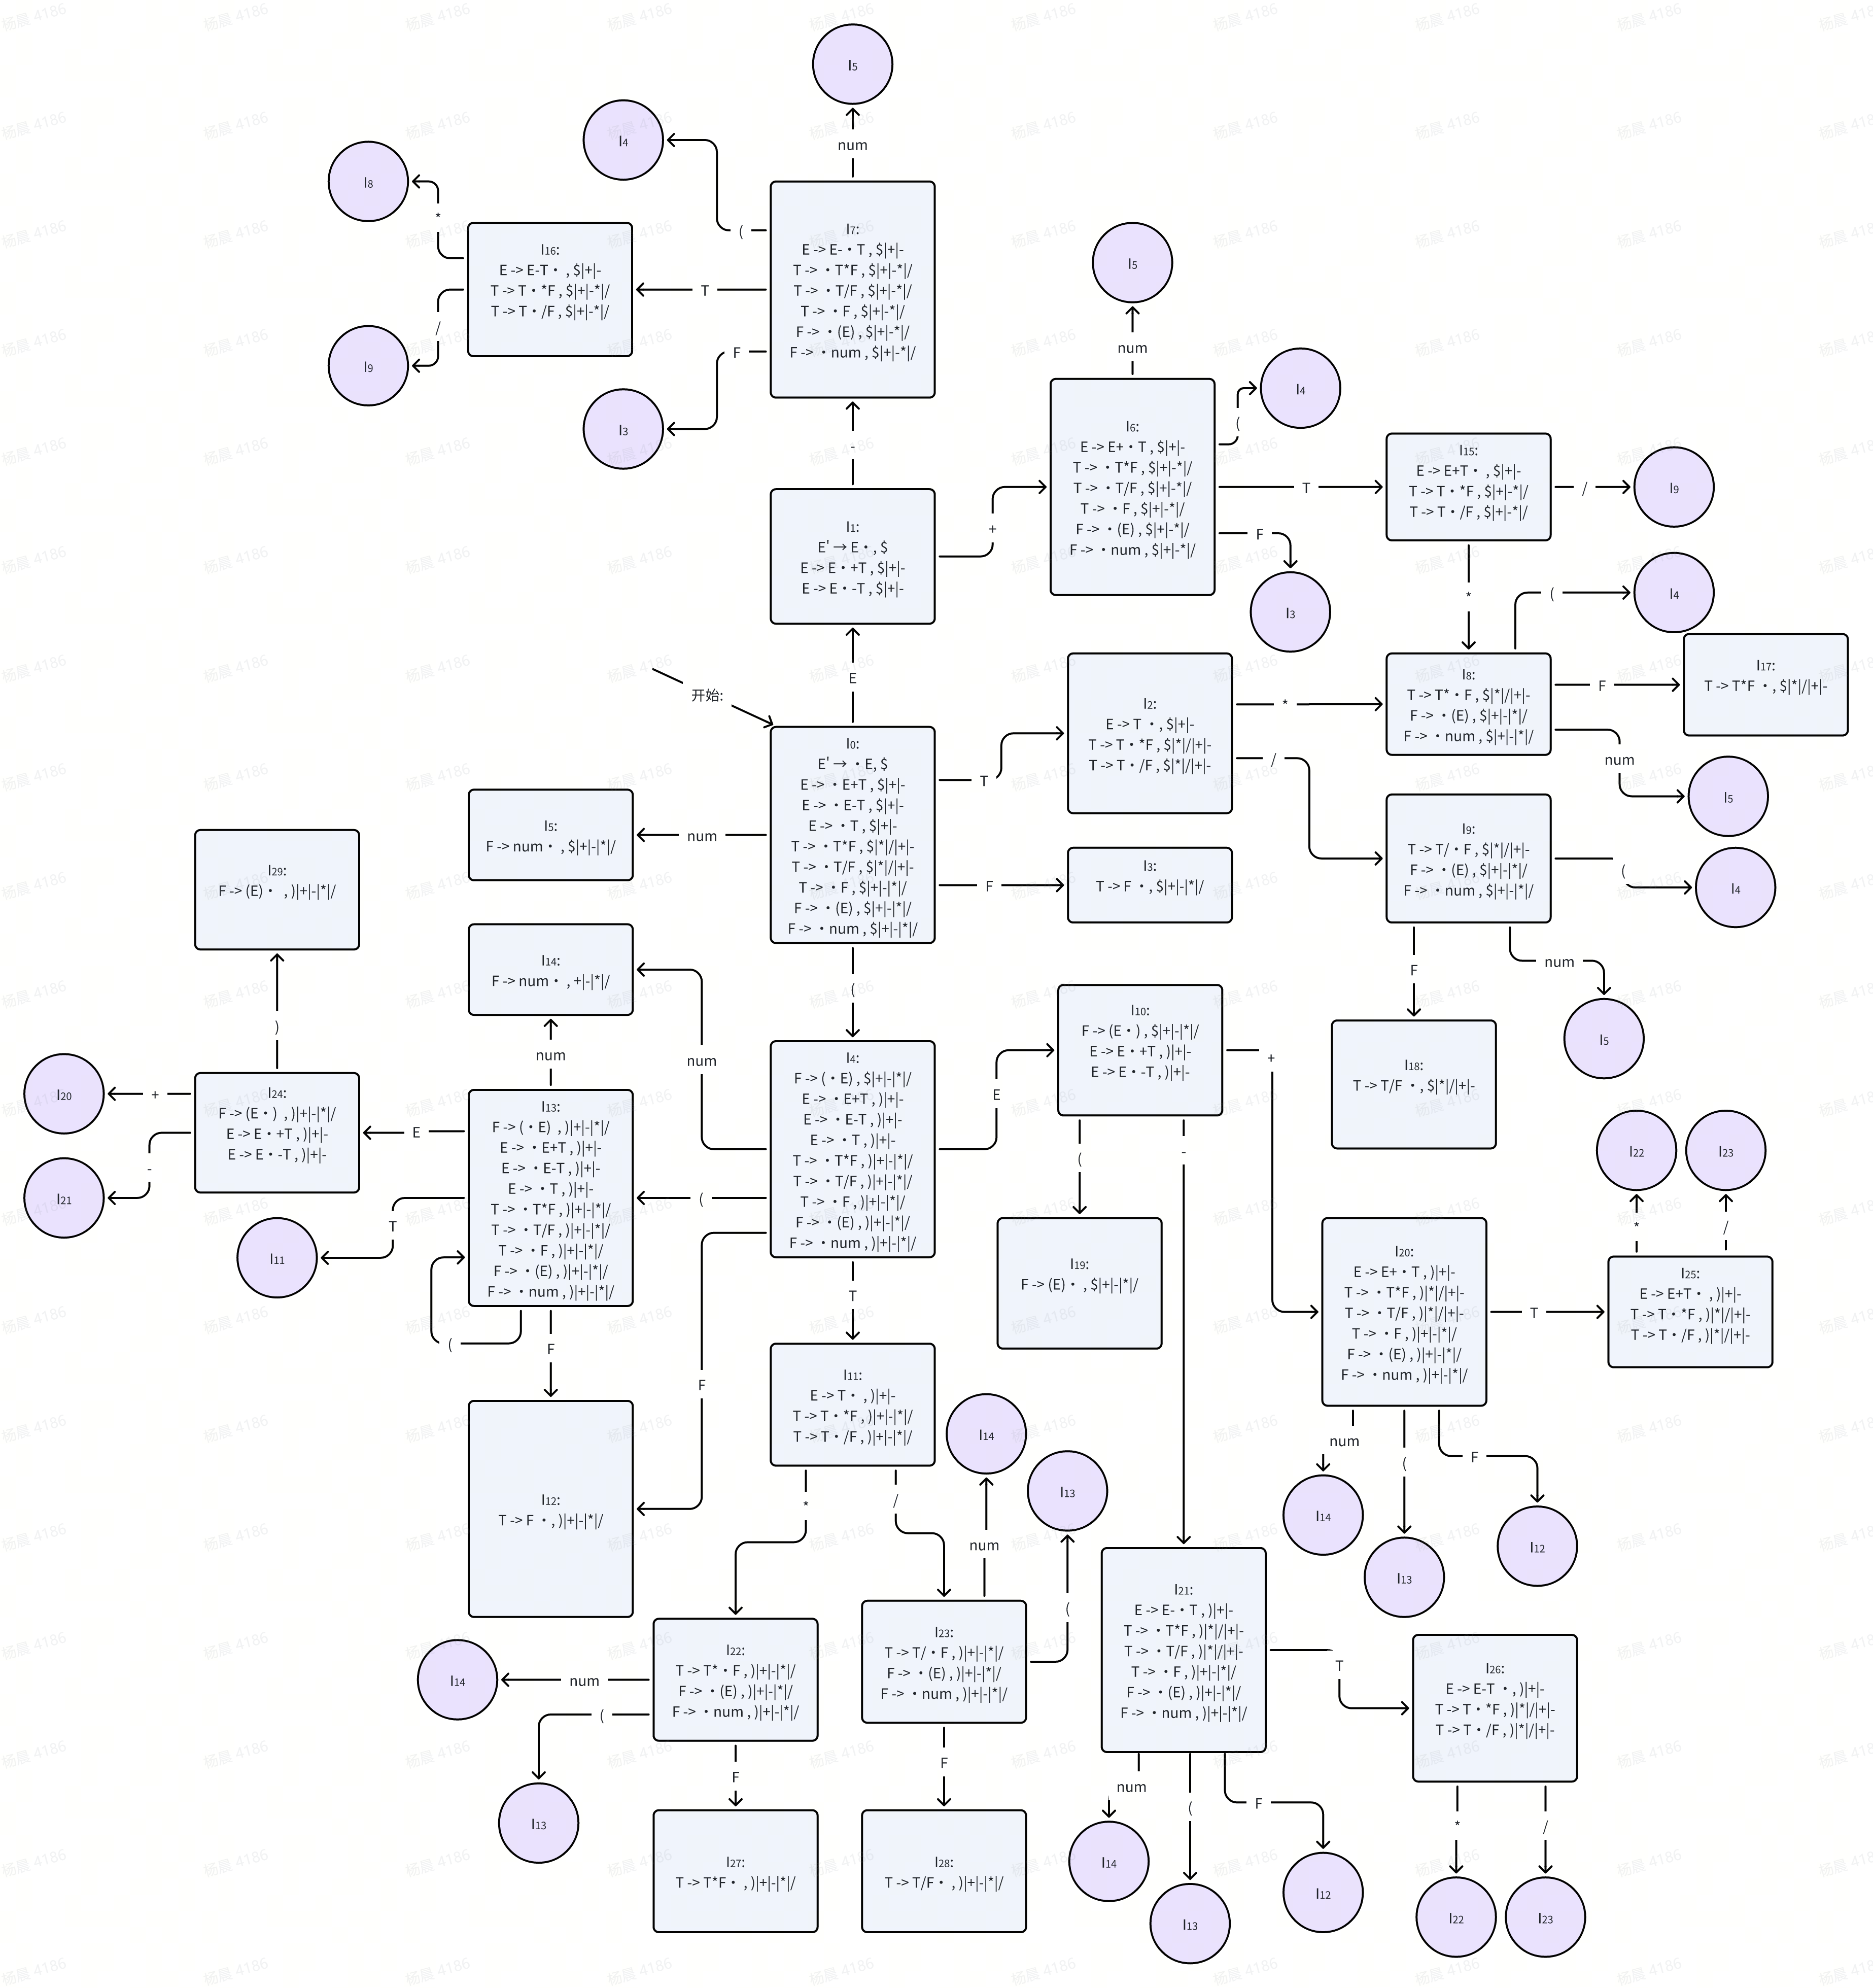
\includegraphics[width=0.9\textwidth]{image/DFA.png}
\caption{识别所有活前缀的DFA}
\end{figure}

\subsection{计算分析表}

根据自动机,可以得到分析表

\begin{lstlisting}
lr1_parser.compute_analysis_table(grammar)
\end{lstlisting}

\subsection{进行LL(1)分析}

在\lstinline{input_string}中给定测试集,然后进行分析

\begin{lstlisting}
input_string = ["1+2", "1+2*(3-(4/0))", "1+2*/(3-4/0))"]
for s in input_string:
    print("输入串:\033[93m{}\033[0m".format(s))
    lr1_parser.parse(grammar, s)
    print('\n')
\end{lstlisting}

分析表如下
\begin{lstlisting}[language=text]
分析表:
状态									action								GOTO
	+		-		*		/		(		)		num		$		E		T		F		
0									S4				S5				1		2		3		
1	S6		S7												ACC								
2	R3		R3		S8		S9								R3								
3	R6		R6		R6		R6								R6								
4									S13				S14				10		11		12		
5	R8		R8		R8		R8								R8								
6									S4				S5						15		3		
7									S4				S5						16		3		
8									S4				S5								17		
9									S4				S5								18		
10	S20		S21								S19												
11	R3		R3		S22		S23				R3												
12	R6		R6		R6		R6				R6												
13									S13				S14				24		11		12		
14	R8		R8		R8		R8				R8												
15	R1		R1		S8		S9								R1								
16	R2		R2		S8		S9								R2								
17	R4		R4		R4		R4								R4								
18	R5		R5		R5		R5								R5								
19	R7		R7		R7		R7								R7								
20									S13				S14						25		12		
21									S13				S14						26		12		
22									S13				S14								27		
23									S13				S14								28		
24	S20		S21								S29												
25	R1		R1		S22		S23				R1												
26	R2		R2		S22		S23				R2												
27	R4		R4		R4		R4				R4												
28	R5		R5		R5		R5				R5												
29	R7		R7		R7		R7				R7												

\end{lstlisting}

\section{测试}

\lstinline{input_string = ["1+2", "1+2*(3-(4/0))", "1+2*/(3-4/0))"]}


\subsection{测试 1+2}
该测试集用于测试一个简单的算数表达式能否被正确识别

\subsubsection{输出结果}

\begin{lstlisting}[language=text]
输入串:(*@\textcolor{orange}{1+2}@*)
Stack                                              	Input                          	Action
State:  0                                         
Symbol: ~                                          	1+2$                          	Shift 5

State:  0 5                                       
Symbol: ~ 1                                        	+2$                           	reduce by F -> num

State:  0 3                                       
Symbol: ~ F                                        	+2$                           	reduce by T -> F

State:  0 2                                       
Symbol: ~ T                                        	+2$                           	reduce by E -> T

State:  0 1                                       
Symbol: ~ E                                        	+2$                           	Shift 6

State:  0 1 6                                     
Symbol: ~ E +                                      	2$                            	Shift 5

State:  0 1 6 5                                   
Symbol: ~ E + 2                                    	$                             	reduce by F -> num

State:  0 1 6 3                                   
Symbol: ~ E + F                                    	$                             	reduce by T -> F

State:  0 1 6 15                                  
Symbol: ~ E +  T                                   	$                             	reduce by E -> E+T

State:  0 1                                       
Symbol: ~ E                                        	$                             	(*@\textcolor{green!60!black}{Acc}@*)
\end{lstlisting}


\subsubsection{输出结果分析}

给定的LR(1)语法分析程序的输出结果表明,输入字符串"1+2\$"符合给定的文法规则。输出结果展示了程序在语法分析过程中的状态转换和操作执行情况。

初始状态为0,程序开始读取输入。通过一系列的Shift和Reduce操作,程序逐步处理输入符号,并根据文法规则进行规约。在每个状态中,程序根据当前输入符号和栈顶的非终结符进行决策,选择执行Shift操作将当前输入符号移入状态栈,或者执行Reduce操作将栈顶的非终结符规约为对应的产生式右侧符号序列。

在最终状态为1时,程序读取到输入符号"\$",并且已完成所有规约操作。此时,程序执行Accept操作,表示输入字符串符合给定的文法规则。

通过输出结果的分析,可以得出结论:输入字符串"1+2"符合给定的文法规则。

\subsection{测试 1+2*(3-(4/0))}

\subsubsection{输出结果}

\begin{lstlisting}[language=text]
输入串:(*@\textcolor{orange}{1+2*(3-(4/0))}@*)
Stack                                              	Input                          	Action
State:  0                                         
Symbol: ~                                          	1+2*(3-(4/0))$                	Shift 5

State:  0 5                                       
Symbol: ~ 1                                        	+2*(3-(4/0))$                 	reduce by F -> num

State:  0 3                                       
Symbol: ~ F                                        	+2*(3-(4/0))$                 	reduce by T -> F

State:  0 2                                       
Symbol: ~ T                                        	+2*(3-(4/0))$                 	reduce by E -> T

State:  0 1                                       
Symbol: ~ E                                        	+2*(3-(4/0))$                 	Shift 6

State:  0 1 6                                     
Symbol: ~ E +                                      	2*(3-(4/0))$                  	Shift 5

State:  0 1 6 5                                   
Symbol: ~ E + 2                                    	*(3-(4/0))$                   	reduce by F -> num

State:  0 1 6 3                                   
Symbol: ~ E + F                                    	*(3-(4/0))$                   	reduce by T -> F

State:  0 1 6 15                                  
Symbol: ~ E +  T                                   	*(3-(4/0))$                   	Shift 8

State:  0 1 6 15 8                                
Symbol: ~ E +  T *                                 	(3-(4/0))$                    	Shift 4

State:  0 1 6 15 8 4                              
Symbol: ~ E +  T * (                               	3-(4/0))$                     	Shift 14

State:  0 1 6 15 8 4 14                           
Symbol: ~ E +  T * (  3                            	-(4/0))$                      	reduce by F -> num

State:  0 1 6 15 8 4 12                           
Symbol: ~ E +  T * (  F                            	-(4/0))$                      	reduce by T -> F

State:  0 1 6 15 8 4 11                           
Symbol: ~ E +  T * (  T                            	-(4/0))$                      	reduce by E -> T

State:  0 1 6 15 8 4 10                           
Symbol: ~ E +  T * (  E                            	-(4/0))$                      	Shift 21

State:  0 1 6 15 8 4 10 21                        
Symbol: ~ E +  T * (  E  -                         	(4/0))$                       	Shift 13

State:  0 1 6 15 8 4 10 21 13                     
Symbol: ~ E +  T * (  E  -  (                      	4/0))$                        	Shift 14

State:  0 1 6 15 8 4 10 21 13 14                  
Symbol: ~ E +  T * (  E  -  (  4                   	/0))$                         	reduce by F -> num

State:  0 1 6 15 8 4 10 21 13 12                  
Symbol: ~ E +  T * (  E  -  (  F                   	/0))$                         	reduce by T -> F

State:  0 1 6 15 8 4 10 21 13 11                  
Symbol: ~ E +  T * (  E  -  (  T                   	/0))$                         	Shift 23

State:  0 1 6 15 8 4 10 21 13 11 23               
Symbol: ~ E +  T * (  E  -  (  T  /                	0))$                          	Shift 14

State:  0 1 6 15 8 4 10 21 13 11 23 14            
Symbol: ~ E +  T * (  E  -  (  T  /  0             	))$                           	reduce by F -> num

State:  0 1 6 15 8 4 10 21 13 11 23 28            
Symbol: ~ E +  T * (  E  -  (  T  /  F             	))$                           	reduce by T -> T/F

State:  0 1 6 15 8 4 10 21 13 11                  
Symbol: ~ E +  T * (  E  -  (  T                   	))$                           	reduce by E -> T

State:  0 1 6 15 8 4 10 21 13 24                  
Symbol: ~ E +  T * (  E  -  (  E                   	))$                           	Shift 29

State:  0 1 6 15 8 4 10 21 13 24 29               
Symbol: ~ E +  T * (  E  -  (  E  )                	)$                            	reduce by F -> (E)

State:  0 1 6 15 8 4 10 21 12                     
Symbol: ~ E +  T * (  E  -  F                      	)$                            	reduce by T -> F

State:  0 1 6 15 8 4 10 21 26                     
Symbol: ~ E +  T * (  E  -  T                      	)$                            	reduce by E -> E-T

State:  0 1 6 15 8 4 10                           
Symbol: ~ E +  T * (  E                            	)$                            	Shift 19

State:  0 1 6 15 8 4 10 19                        
Symbol: ~ E +  T * (  E  )                         	$                             	reduce by F -> (E)

State:  0 1 6 15 8 17                             
Symbol: ~ E +  T *  F                              	$                             	reduce by T -> T*F

State:  0 1 6 15                                  
Symbol: ~ E +  T                                   	$                             	reduce by E -> E+T

State:  0 1                                       
Symbol: ~ E                                        	$                             	(*@\textcolor{green!60!black}{Acc}@*)
\end{lstlisting}

\subsubsection{输出结果分析}

通过一系列的状态转换和操作执行,程序成功地完成了对输入字符串"1+2*(3-(4/0))"的语法分析。

在初始状态为0时,程序开始读取输入符号,并根据当前输入符号和栈顶的非终结符进行决策。通过一系列的Shift和Reduce操作,程序逐步处理输入符号,并根据文法规则进行规约。

最终状态为1,表示程序已经读取完整个输入字符串,并且完成了所有的规约操作。此时,程序执行Accept操作,表示输入字符串符合给定的文法规则。

通过输出结果的分析,可以得出结论:输入字符串"1+2*(3-(4/0))"符合给定的文法规则。程序成功地执行了语法分析,并验证了输入字符串的语法正确性。

\subsection{测试 1+2*/(3-4/0))}

\subsubsection{输出结果}

\begin{lstlisting}[language=text]
输入串:(*@\textcolor{orange}{1+2*/(3-4/0))}@*)
Stack                                              	Input                          	Action
State:  0                                         
Symbol: ~                                          	1+2*/(3-4/0))$                	Shift 5

State:  0 5                                       
Symbol: ~ 1                                        	+2*/(3-4/0))$                 	reduce by F -> num

State:  0 3                                       
Symbol: ~ F                                        	+2*/(3-4/0))$                 	reduce by T -> F

State:  0 2                                       
Symbol: ~ T                                        	+2*/(3-4/0))$                 	reduce by E -> T

State:  0 1                                       
Symbol: ~ E                                        	+2*/(3-4/0))$                 	Shift 6

State:  0 1 6                                     
Symbol: ~ E +                                      	2*/(3-4/0))$                  	Shift 5

State:  0 1 6 5                                   
Symbol: ~ E + 2                                    	*/(3-4/0))$                   	reduce by F -> num

State:  0 1 6 3                                   
Symbol: ~ E + F                                    	*/(3-4/0))$                   	reduce by T -> F

State:  0 1 6 15                                  
Symbol: ~ E +  T                                   	*/(3-4/0))$                   	Shift 8

State:  0 1 6 15 8                                
Symbol: ~ E +  T *                                 	/(3-4/0))$                    	 (*@\textcolor{red}{error(s)}@*) 
\end{lstlisting}

\subsubsection{输出结果分析}

根据给定的LR(1)语法分析程序的输出结果,可以总结如下:

在进行语法分析时,输入字符串"1+2*/(3-4/0))"在状态栈为0 1 6 15 8时出现了错误。

在此状态下,程序读取到输入符号"*",但栈顶的非终结符为T。根据给定的文法规则,"*"不是T的后继符号,因此无法进行后续操作。这导致了语法分析的错误。

通过输出结果的分析,可以得出结论:输入字符串"1+2*/(3-4/0))"不符合给定的文法规则。程序在语法分析过程中出现了错误,提示了输入字符串中的语法错误。

在这种情况下,需要检查输入字符串中的语法错误,例如检查运算符的使用是否正确、括号是否匹配等。修正输入字符串中的错误后,再次进行语法分析以验证其正确性。

\section{实验总结}

在本次实验中,我编写了一个简单的LR(1)语法分析程序,它帮助我更清楚地理解了自底向上语法分析的流程,并加深了对相关知识点的掌握。

该程序的架构相对简单,主要难点在于数据结构的设计和算法的实现。特别是LR(1)项目和项目集的表示方式需要既准确又易于计算,这增加了实现的复杂性。在编写过程中,我利用了Python语言的特性,使算法过程更加清晰,大大降低了编程的复杂度。

然而,我的语法分析程序仍然有许多改进的空间,尤其是在错误处理方面。目前的程序对错误的处理不够全面,需要进一步改进以提高其健壮性。

通过这次实验,我不仅对课堂上学到的知识有了更深入的理解,还提升了我的Python编程能力。这次经历让我受益匪浅,收获颇多。
% \subsection{全局选项}
% 此模板定义了一个语言选项 \lstinline{lang},可以选择英文模式 \lstinline{lang=en}(默认)或者中文模式 \lstinline{lang=cn}。当选择中文模式时,图表的标题引导词以及参考文献,定理引导词等信息会变成中文。你可以通过下面两种方式来选择语言模式:
% \begin{lstlisting}
% \documentclass[lang=cn]{elegantpaper} % or
% \documentclass{cn}{elegantpaper} 
% \end{lstlisting}

% \textbf{注意:} 英文模式下,由于没有添加中文宏包,无法输入中文。如果需要输入中文,可以通过在导言区引入中文宏包 \lstinline{ctex} 或者加入 \lstinline{xeCJK} 宏包后自行设置字体。 
% \begin{lstlisting}
% \usepackage[UTF8,scheme=plain]{ctex}
% \end{lstlisting}

% \subsection{数学字体选项}

% 本模板定义了一个数学字体选项(\lstinline{math}),可选项有三个:
% \begin{enumerate}
%   \item \lstinline{math=cm}(默认),使用 \LaTeX{} 默认数学字体(推荐,无需声明);
%   \item \lstinline{math=newtx},使用 \lstinline{newtxmath} 设置数学字体(潜在问题比较多)。
%   \item \lstinline{math=mtpro2},使用 \lstinline{mtpro2} 宏包设置数学字体,要求用户已经成功安装此宏包。
% \end{enumerate}

% \subsection{中文字体选项}

% 模板提供中文字体选项 \lstinline{chinesefont},可选项有
% \begin{enumerate}
%   \item \lstinline{ctexfont}:默认选项,使用 \lstinline{ctex} 宏包根据系统自行选择字体,可能存在字体缺失的问题,更多内容参考 \lstinline{ctex} 宏包\href{https://ctan.org/pkg/ctex}{官方文档}\footnote{可以使用命令提示符,输入 \lstinline{texdoc ctex} 调出本地 \lstinline{ctex} 宏包文档}。
%   \item \lstinline{founder}:方正字体选项(\textbf{需要安装方正字体}),后台调用 \lstinline{ctex} 宏包并且使用 \lstinline{fontset=none} 选项,然后设置字体为方正四款免费字体,方正字体下载注意事项见后文,用户只需要安装方正字体即可使用该选项。
%   \item \lstinline{nofont}:后台会调用 \lstinline{ctex} 宏包并且使用 \lstinline{fontset=none} 选项,不设定中文字体,用户可以自行设置中文字体,具体见后文。
% \end{enumerate}

% \subsubsection{方正字体选项}
% 由于使用 \lstinline{ctex} 宏包默认调用系统已有的字体,部分系统字体缺失严重,因此,用户希望能够使用其它字体,我们推荐使用方正字体。方正的{\songti 方正书宋}、{\heiti 方正黑体}、{\kaishu 方正楷体}、{\fangsong 方正仿宋}四款字体均可免费试用,且可用于商业用途。用户可以自行从\href{http://www.foundertype.com/}{方正字体官网}下载此四款字体,在下载的时候请\textbf{务必}注意选择 GBK 字符集,也可以使用 \href{https://www.latexstudio.net/}{\LaTeX{} 工作室}提供的\href{https://pan.baidu.com/s/1BgbQM7LoinY7m8yeP25Y7Q}{方正字体,提取码为:njy9} 进行安装。安装时,{\kaishu Win 10 用户请右键选择为全部用户安装,否则会找不到字体。}

% \begin{figure}[!htb]
% \centering
% 
\includegraphics[width=0.9\textwidth]{founder.png}
% \end{figure}

% \subsubsection{其他中文字体}
% 如果你想完全自定义字体\footnote{这里仍然以方正字体为例。},你可以选择 \lstinline{chinesefont=nofont},然后在导言区设置即可,可以参考下方代码:
% \begin{lstlisting}
% \setCJKmainfont[BoldFont={FZHei-B01},ItalicFont={FZKai-Z03}]{FZShuSong-Z01}
% \setCJKsansfont[BoldFont={FZHei-B01}]{FZKai-Z03}
% \setCJKmonofont[BoldFont={FZHei-B01}]{FZFangSong-Z02}
% \setCJKfamilyfont{zhsong}{FZShuSong-Z01}
% \setCJKfamilyfont{zhhei}{FZHei-B01}
% \setCJKfamilyfont{zhkai}[BoldFont={FZHei-B01}]{FZKai-Z03}
% \setCJKfamilyfont{zhfs}[BoldFont={FZHei-B01}]{FZFangSong-Z02}
% \newcommand*{\songti}{\CJKfamily{zhsong}}
% \newcommand*{\heiti}{\CJKfamily{zhhei}}
% \newcommand*{\kaishu}{\CJKfamily{zhkai}}
% \newcommand*{\fangsong}{\CJKfamily{zhfs}}
% \end{lstlisting}



% \subsection{自定义命令}
% 此模板并没有修改任何默认的 \LaTeX{} 命令或者环境\footnote{目的是保证代码的可复用性,请用户关注内容,不要太在意格式,这才是本工作论文模板的意义。}。另外,我自定义了 4 个命令:
% \begin{enumerate}
%   \item \lstinline{\email}:创建邮箱地址的链接,比如 \email{ddswhu@outlook.com};
%   \item \lstinline{\figref}:用法和 \lstinline{\ref} 类似,但是会在插图的标题前添加 <\textbf{图 n}> ;
%   \item \lstinline{\tabref}:用法和 \lstinline{\ref} 类似,但是会在表格的标题前添加 <\textbf{表 n}>;
%   \item \lstinline{\keywords}:为摘要环境添加关键词。
% \end{enumerate}

% \subsection{参考文献}

% 文献部分,本模板调用了 biblatex 宏包,并提供了 biber(默认) 和 bibtex 两个后端选项,可以使用 \lstinline{bibend} 进行修改:

% \begin{lstlisting}
%   \documentclass[bibtex]{elegantpaper}
%   \documentclass[bibend=bibtex]{elegantpaper}
% \end{lstlisting}

% 关于文献条目(bib item),你可以在谷歌学术,Mendeley,Endnote 中取,然后把它们添加到 \lstinline{reference.bib} 中。在文中引用的时候,引用它们的键值(bib key)即可。

% 为了方便文献样式修改,模板引入了 \lstinline{bibstyle} 和 \lstinline{citestyle} 选项,默认均为数字格式(numeric),参考文献示例:\cite{cn1,en2,en3} 使用了中国一个大型的 P2P 平台(人人贷)的数据来检验男性投资者和女性投资者在投资表现上是否有显著差异。

% 如果需要设置为国标 GB7714-2015,需要使用:
% \begin{lstlisting}
%   \documentclass[citestyle=gb7714-2015, bibstyle=gb7714-2015]{elegantpaper} 
% \end{lstlisting}

% 如果需要添加排序方式,可以在导言区加入
% \begin{lstlisting}
%   \ExecuteBibliographyOptions{sorting=ynt}
% \end{lstlisting}

% 启用国标之后,可以加入 \lstinline{sorting=gb7714-2015}。


% \section{使用 newtx 系列字体}

% 如果需要使用原先版本的 \lstinline{newtx} 系列字体,可以通过显示声明数学字体:

% \begin{lstlisting}
% \documentclass[math=newtx]{elegantpaper}
% \end{lstlisting}

% \subsection{连字符}

% 如果使用 \lstinline{newtx} 系列字体宏包,需要注意下连字符的问题。
% \begin{equation}
%   \int_{R^q} f(x,y) dy.\emph{of\kern0pt f}
% \end{equation}

% \begin{lstlisting}
% \begin{equation}
%   \int_{R^q} f(x,y) dy.\emph{of \kern0pt f}
% \end{equation}
% \end{lstlisting}

% \subsection{宏包冲突}

% 有用户反馈模板在使用 \lstinline{yhmath} 以及 \lstinline{esvect} 等宏包时会报错:
% \begin{lstlisting}
% LaTeX Error:
%    Too many symbol fonts declared.
% \end{lstlisting}

% 原因是在使用 \lstinline{newtxmath} 宏包时,重新定义了数学字体用于大型操作符,达到了 {\heiti 最多 16 个数学字体} 的上限,在调用其他宏包的时候,无法新增数学字体。为了减少调用非常用宏包,在此给出如何调用 \lstinline{yhmath} 以及 \lstinline{esvect} 宏包的方法。

% 请在 \lstinline{elegantpaper.cls} 内搜索 \lstinline{yhmath} 或者 \lstinline{esvect},将你所需要的宏包加载语句\textit{取消注释}即可。


% \section{常见问题 FAQ}

% \begin{enumerate}[label=\arabic*).]
%   \item \textit{如何删除版本信息?}\\
%     导言区不写 \lstinline|\version{x.xx}| 即可。
%   \item \textit{如何删除日期?}\\
%     需要注意的是,与版本 \lstinline{\version} 不同的是,导言区不写或注释 \lstinline{\date} 的话,仍然会打印出当日日期,原因是 \lstinline{\date} 有默认参数。如果不需要日期的话,日期可以留空即可,也即 \lstinline|\date{}|。
%   \item \textit{如何获得中文日期?}\\
%     为了获得中文日期,必须在中文模式下\footnote{英文模式下,由于未加载中文宏包,无法输入中文。},使用 \lstinline|\date{\zhdate{2019/10/11}}|,如果需要当天的汉化日期,可以使用 \lstinline|\date{\zhtoday}|,这两个命令都来源于 \href{https://ctan.org/pkg/zhnumber}{\lstinline{zhnumber}} 宏包。
%   \item \textit{如何添加多个作者?}\\
%     在 \lstinline{\author} 里面使用 \lstinline{\and},作者单位可以用 \lstinline{\\} 换行。
%     \begin{lstlisting}
%     \author{author 1\\ org. 1 \and author 2 \\ org. 2 }
%     \end{lstlisting}
%   \item \textit{如何添加中英文摘要?}\\
%     请参考 \href{https://github.com/ElegantLaTeX/ElegantPaper/issues/5}{GitHub::ElegantPaper/issues/5}
% \end{enumerate}


% \section{致谢}

% 特别感谢 \href{https://github.com/sikouhjw}{sikouhjw} 和 \href{https://github.com/syvshc}{syvshc}  长期以来对于 Github 上 issue 的快速回应,以及各个社区论坛对于 ElegantLaTeX 相关问题的回复。特别感谢 ChinaTeX 以及 \href{http://www.latexstudio.net/}{LaTeX 工作室} 对于本系列模板的大力宣传与推广。

% 如果你喜欢我们的模板,你可以在 Github 上收藏我们的模板。

% \nocite{*}
% \printbibliography[heading=bibintoc, title=\ebibname]

% \appendix
% %\appendixpage
% \addappheadtotoc

\end{document}
